\documentclass[11pt,a4paper]{article}
\usepackage[latin1]{inputenc}
\usepackage[top=1in,bottom=1in,left=0.75in,right=0.75in]{geometry}
\usepackage{amsmath}
\usepackage{soul}
\usepackage{hyperref}
\usepackage{listings}
\usepackage{lastpage} % for the number of the last page in the document
\usepackage{fancyhdr}
\pagestyle{fancy}
\usepackage{graphicx}
\usepackage[table]{xcolor}
\usepackage{framed}
\usepackage{tabularx}
\setlength\parindent{0cm}
\setlength{\parskip}{0.15cm}%
\usepackage{longtable}
\usepackage{wrapfig}
\fancyhf{}
\fboxrule=4pt%border thickness
\lhead{Documentation}
\rhead{Project Plan}
\usepackage{graphicx}
\usepackage{subfig}

\lfoot{}
\rfoot{Page \thepage\ of \pageref{LastPage}}\usepackage{amsfonts}
\usepackage{amssymb}

\begin{document}
\pagenumbering{gobble}

\pagenumbering{gobble}
\begin{titlepage}

\newcommand{\HRule}{\rule{\linewidth}{0.5mm}} % Defines a new command for the horizontal lines, change thickness here

\center % Center everything on the page


\includegraphics[scale=0.4]{images/aber.png} \\[1.5cm] % Name of your university/college
\textsc{\Large Aberystwyth University
 \\[0.5cm] Department of Computer Science}

\

\textsc{\Large Project AWESOME}\\

\HRule \\[0.4cm]
{ \huge  Project Plan}\\[0.4cm] % Title of your document
\HRule \\[1.5cm]

\Large \emph{Author:}\\
Keiron \textsc{O'Shea (keo7@aber.ac.uk)}\\[1cm] % Your name 

{\large June 2014}\\[2cm] % Date, change the \today to a set date if you want to be precise

\


\small version: 0.02 \\
\small status: draft


\vfill % Fill the rest of the page with whitespace

\end{titlepage}

\thispagestyle{plain}	

\tableofcontents

\clearpage

\pagenumbering{arabic}

\clearpage

\section{Introduction}

\subsection{Purpose of this document}


The purpose of this document is to present how I've translated the project brief, the Aberystwyth Web Evaluation Surveys Of Module Experiences (AWESOME), a web-based module evaluation questionnaire generator for the monitoring and evaluation of teaching, into subsystems of objectives and milestones.

Moreover this document will describe the various interactions between separate components of the system and outline initial ideas surrounding the visual appearance of the user interface.

This document will also discuss project management with the use of a Gantt Chart, providing an overview of the project's major tasks and related milestones. This will coexist with a probabilistic analysis of risks, of which will cover some main issues that may occur throughout the development of the project.

\subsection{Scope}

The project plan should intend to give an overview of the proposed system, including a brief description of platforms and HLA - as well as provide a description of target users. It will also contain a user case diagram that aims to give an overview of how the users might interact with each-other. An idea of the user-interface design will also be provided with descriptions of how it will interact with the end user. In terms of project management, a Gantt chart will be used to display the start and end dates fo rthe main tasks of the project and a risk analysis that will highlight issues the project may encounter.

\subsection{Objectives}

The objectives of this particular document are:

\begin{itemize}
	\item to describe the appearance of the user interface.
	\item to indicate an understanding of user behaviour.
	\item give further indication of the proposed time-line surrounding the development of the project.
	\item to indicate an understanding of the risks and other factors of the project.
\end{itemize}

\clearpage

\section{Overview}

The "Aberystwyth Web Evaluation Surveys Of Module Experiences", or AWESOME for short, is a web-based module evaluation questionnaire generator for the monitoring and evaluation of teaching.

\subsection{Platforms and High Level Architecture}

I intend to use the following platforms for the system.

\subsubsection{Hypertext Markup Language (HTML)}

The project brief stated specifically that the system is to be deployed completely via the web. We will be using  Hypertext Markup Language (HTML) as the markup language used to create the application.

\subsubsection{Cascading Style Sheets (CSS)}

In order to produce an aesthetically-pleasing web application I will utilise CSS to specify the styles of the visual elements of the website.

\subsubsection{PHP: Hypertext Preprocessor (PHP)}

On the server side PHP will be used to handle communication between the client and the database and handle the creation of the questionnaires as well as providing dynamic web pages. PHP is widely available on the majority (if not all) web servers and is relatively easy to deploy compared to similar systems.

\subsubsection{PostgreSQL}

PostgreSQL is one of the most widely used database platforms and will be used to store application information. The platform is renowned for its simplistic commands and is easily deployed and managed.

\

The high level architecture consists of the following elements and application mechanics;

\subsubsection{Analytics}

For staff to analyse feedback analytics consisting of visually-appealing graphs and textual responses will be rendered.

\subsubsection{Internet Connectivity}

Both staff and students will require connection to the server to allow them to use the application. Google Charts has been pinpointed as a possible way of doing this as it comes with a readily available API, and still keeps in line with the approach of using free software to build the entire system.

\subsubsection{Staff Login}

\subsubsection{Staff Access to SAMS/AStRA}

\subsection{Description of Target Users}

All design must begin with the understanding of who the user is, but due to the relatively large range of age and expertise of the target-base this will be difficult to achieve. The proposed system will be targeted to both staff and students who are currently working or studying at a higher education institute. Because of this inability to pinpoint a specific user base, it would be best to ensure that when designing the user interface we need to ensure that the application is simple to use (in order to avoid frustration and confusing) it must also be informative.

\subsection{Software Licensing}

\begin{framed}
\begin{verbatim}
Permission is hereby granted, free of charge, to any person obtaining a copy
of this software and associated documentation files (the "Software"), to deal
in the Software without restriction, including without limitation the rights
to use, copy, modify, merge, publish, distribute, sublicense, and/or sell
copies of the Software, and to permit persons to whom the Software is
furnished to do so, subject to the following conditions:

The above copyright notice and this permission notice shall be included in
all copies or substantial portions of the Software.

THE SOFTWARE IS PROVIDED "AS IS", WITHOUT WARRANTY OF ANY KIND, EXPRESS OR
IMPLIED, INCLUDING BUT NOT LIMITED TO THE WARRANTIES OF MERCHANTABILITY,
FITNESS FOR A PARTICULAR PURPOSE AND NONINFRINGEMENT. IN NO EVENT SHALL THE
AUTHORS OR COPYRIGHT HOLDERS BE LIABLE FOR ANY CLAIM, DAMAGES OR OTHER
LIABILITY, WHETHER IN AN ACTION OF CONTRACT, TORT OR OTHERWISE, ARISING FROM,
OUT OF OR IN CONNECTION WITH THE SOFTWARE OR THE USE OR OTHER DEALINGS IN
THE SOFTWARE.
\end{verbatim}
\end{framed}

\clearpage

\section{Use Case}


\subsection{Use Case Diagram}

\subsection{Use Case Descriptions}
\clearpage
\section{User interface design}

\subsection{User Navigation}

\subsection{GUI Design}

The following images cover the initial concept of the application. These mockups were completed using the GNU Image Manipulation Program (GIMP) allowing for editing on evaluation.

\subsubsection{Home Page}

\begin{figure}[hbtp]
\centering
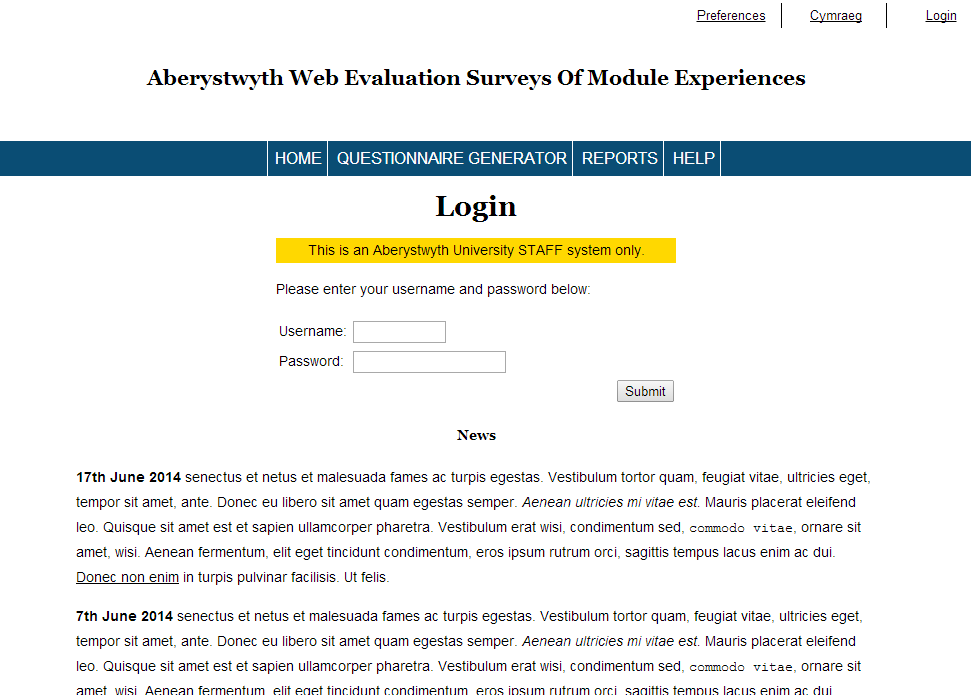
\includegraphics[width=0.85\linewidth]{images/uidesign/homepage.png}
\end{figure}


\clearpage
\section{Project Management}

\subsection{Gantt Chart}

The below figure is a Gantt chart, a visual representation of the project schedule. It describes the project milestones and task dependencies.

\subsection{Risk Analysis}

\clearpage

\section*{Document History}

\begin{center}
\begin{tabular}{|c | c | c | c | c |}
\hline
\textbf{Version} \cellcolor{gray!25} & \textbf{Date} \cellcolor{gray!25}& \cellcolor{gray!25}\textbf{Changes made to Document} &\textbf{ Changed by} \cellcolor{gray!25}\\
\hline
0.2 & 17-06-2014 & Completed overview & KeironO \\
\hline
0.1 & 16-06-2014 & Initial creation & KeironO \\
\hline

\hline
\end{tabular}
\end{center}
\clearpage


\end{document}
